\documentclass[9pt,aspectratio=169]{beamer}


\usepackage{tabu, booktabs, multirow}
\usepackage{tabularx}
\usepackage{multicol}
\usepackage{setspace}
\usepackage[official]{eurosym}
\usepackage{graphicx}

\usepackage{hyperref}
\hypersetup{
    colorlinks=true,
    linkcolor=blue,
    filecolor=magenta,      
    urlcolor=cyan,
    pdftitle={EC3318/MN3101 Lecture 1 2026/27},
    pdfpagemode=FullScreen,
    }

\urlstyle{same}

\graphicspath{ {./pix_l1/} }



\newcolumntype{Y}{>{\centering\arraybackslash}X}  % Centered version of X

\newcommand{\placeholderbox}[1]{%
  \begin{center}
    \fbox{\parbox[c][0.5\textheight][c]{0.9\linewidth}{\centering \textit{#1}}}
  \end{center}
}
% St Andrews Color Palette

% Blues
\definecolor{StAndrewsLightBlue}{RGB}{0,174,239}
\definecolor{StAndrewsMidBlue}{RGB}{0,125,197}
\definecolor{StAndrewsBlue}{RGB}{0,83,155}  % Previously defined

% Reds
\definecolor{StAndrewsBurgundy}{RGB}{198,12,70}
\definecolor{StAndrewsRed}{RGB}{238,49,42}  % Previously defined

% Purple
\definecolor{StAndrewsPurple}{RGB}{123,67,154}

% Orange
\definecolor{StAndrewsOrange}{RGB}{245,132,43}

% Greens
\definecolor{StAndrewsGreen}{RGB}{84,185,72}
\definecolor{StAndrewsMidGreen}{RGB}{0,133,63}
\definecolor{StAndrewsDarkGreen}{RGB}{0,89,83}

% Yellow
\definecolor{StAndrewsYellow}{RGB}{255,223,0}

% Black
\definecolor{StAndrewsBlack}{RGB}{35,31,32}

\setbeamercolor*{structure}{fg=StAndrewsBlack}
\setbeamercolor{title}{fg=StAndrewsBlack}
\setbeamercolor{title separator}{fg=StAndrewsBlue}
\setbeamercolor{frametitle}{bg=StAndrewsBlue, fg=white}

\usetheme{metropolis}
\usepackage{tikz}
\usetikzlibrary{calc}
\usetikzlibrary{arrows.meta, positioning, shapes.geometric, shadows}
\usepackage[export]{adjustbox}
\usepackage{hyperref}
\hypersetup{
  colorlinks=true,
  linkcolor=StAndrewsBlue,
  urlcolor=StAndrewsBlue,
  citecolor=StAndrewsBlue
}

% Show a full-width colored header with title + subtitle
\setbeamercolor{frametitle}{bg=StAndrewsBlue, fg=white}
\setbeamercolor{framesubtitle}{fg=white}
\setbeamerfont{frametitle}{size=\Large,series=\mdseries}
\setbeamerfont{title}{series=\mdseries}
\setbeamerfont{framesubtitle}{size=\small}

\makeatletter
\setbeamertemplate{frametitle}{
  \nointerlineskip
  % Preserve the original header padding; ex changes slightly with font weight.
  \begin{beamercolorbox}[wd=\paperwidth,sep=4.6165pt,leftskip=1.2em,rightskip=1.2em]{frametitle}
    \usebeamerfont{frametitle}\strut\insertframetitle\par
    \ifx\insertframesubtitle\@empty\else
      \vspace{0.25ex}
      {\usebeamerfont{framesubtitle}\usebeamercolor[fg]{framesubtitle}\insertframesubtitle\par}
    \fi
  \end{beamercolorbox}
}
\makeatother

\makeatletter
\setbeamertemplate{title page}{
  \begin{minipage}[c][\textheight][c]{\textwidth}
    \centering
    \ifx\inserttitle\@empty\else\usebeamertemplate*{title}\fi
    \ifx\insertsubtitle\@empty\else\usebeamertemplate*{subtitle}\fi
    \vspace{8pt}
    {\usebeamercolor[fg]{title separator}\rule{0.72\textwidth}{0.4pt}\par}
    \vspace{10pt}
    \ifx\beamer@shortauthor\@empty\else\usebeamertemplate*{author}\fi
    \vspace{12pt}
    \ifx\insertinstitute\@empty\else\usebeamertemplate*{institute}\fi
    \vspace{6pt}
    \ifx\insertdate\@empty\else\usebeamertemplate*{date}\fi
    \vspace{9pt}
    \ifx\inserttitlegraphic\@empty\else\usebeamertemplate*{title graphic}\fi
  \end{minipage}
}

\setbeamertemplate{title}{
%  \raggedright%  % <-- Comment here
  \linespread{1.0}%
  \inserttitle%
  \par%
}
\setbeamertemplate{subtitle}{
%  \raggedright%  % <-- Comment here
  \insertsubtitle%
  \par%
  \vspace*{0.5em}
}
\setbeamertemplate{author}{
%  \raggedright%  % <-- Comment here
  \insertauthor%
  \par%
}
\setbeamertemplate{institute}{\insertinstitute\par}
\makeatother

\title{\LARGE Lecture 1: \\
Discounting, compounding and investment appraisal}
\author[Dr Christian Engels]{Dr Christian Engels}
\institute{\small{EC3318 Financial Economics: Corporate Finance \\ MN3101 Corporate Finance and Control \\[2mm] University of St Andrews Business School}}
\date{15 September 2026}


\newenvironment{wideitemize}{\itemize\addtolength{\itemsep}{10pt}}{\enditemize}
\setbeamertemplate{items}[circle]

\setbeamertemplate{title graphic}{\inserttitlegraphic\par}
\titlegraphic{
\includegraphics[scale=0.08]{logos/01-standard-black-text.png}}

% Add the logo to the bottom left
\addtobeamertemplate{footline}{%
  \begin{tikzpicture}[remember picture,overlay]
    \node[anchor=south west, inner sep=0pt] at ([xshift=0.5cm, yshift=0.25cm]current page.south west) {
      
\includegraphics[height=0.5cm]{logos/st-andrews-icon.png}
    };
  \end{tikzpicture}%
}{}


\usepackage{pgfplots}
\pgfplotsset{compat=1.18}
\newcommand{\UnclePV}{21,082.90}
\newcommand{\UncleFV}{24,440.86}
\newcommand{\OfficeNPV}{57,236.67}
\newcommand{\OfficeIRR}{10.48}
\newcommand{\CrossRate}{9.49}
\newcommand{\DoubleNPV}{114,473.34}
\newcommand{\CoalLowIRR}{3.09}
\newcommand{\CoalHighIRR}{25.16}
\newcommand{\CoalNPV}{5.89}
\newcommand{\CoalAdjustedIRR}{22.05}
\newcommand{\CoalMIRR}{20.38}
\newcommand{\CoalPVminus}{370.75}
\newcommand{\CoalFVplus}{937.20}
\newcommand{\MineNPV}{26.85}
\newcommand{\MineIn}{125.19}
\newcommand{\MineOut}{152.04}
\newcommand{\DiscountedPB}{2.53}
\newcommand{\InterpPositive}{17,992.95}
\newcommand{\InterpNegative}{738.99}
\newcommand{\InterpFall}{18,731.94}
\newcommand{\InterpFractionPercent}{96.05}
\newcommand{\InterpFractionDecimal}{0.960549}
\newcommand{\InterpRateIncrease}{0.4803}
\newcommand{\InterpRateFour}{10.4803}
\newcommand{\InterpRateFive}{10.48027}
\newcommand{\InterpRootFive}{10.47998}
\newcommand{\InterpResidualWhole}{11}
\newcommand{\InterpRatePosition}{9.6054909988}
\newcommand{\InterpToyPosition}{7.5000000000}

\newcommand{\source}[1]{\par\smallskip{\footnotesize\color{StAndrewsBlack}#1\par}}
\pgfplotsset{lectureplot/.style={width=10.6cm,height=4.35cm,
 axis lines=left, tick label style={font=\footnotesize},
 label style={font=\small},scaled ticks=false,
 tick align=outside, clip=false, axis line style={black!55},
 every axis plot/.append style={thick,no marks}}}
\begin{document}
\frame[plain]{\titlepage}

\begin{frame}{Content of today's lecture}
\begin{columns}[t]
  \begin{column}{0.49\textwidth}
    \tableofcontents[sections={1}]
  \end{column}
  \begin{column}{0.49\textwidth}
    \tableofcontents[sections={2}]
  \end{column}
\end{columns}
\end{frame}

\section[Part 1: Discounting and Compounding]{\textbf{Part 1: Discounting and Compounding}}

\subsection{Reading}

\begin{frame}{Required reading}
\begin{enumerate}
\item Hillier, D., Ross, S., Westerfield, R., Jaffe, J. \& Jordan, B. (2020) Corporate Finance. 4th ed. London: McGraw-Hill Education. ISBN-13: 9781526848086. Chapter 4.
\item Brealey, R. A., Myers, S. C., Allen, F., \& Edmans, A. (2023). Principles of Corporate Finance (14th ed.). McGraw-Hill Education. Chapter 2: How to Calculate Present Values.
\item Ruback, R.S. (2011) Downsides and DCF: Valuing Biased Cash Flow Forecasts. \textit{Journal of Applied Corporate Finance} 23, 8-17. \href{https://doi.org/10.1111/j.1745-6622.2011.00322.x}{https://doi.org/10.1111/j.1745-6622.2011.00322.x}
\end{enumerate}
\end{frame}

\subsection{Interest Rate}

\begin{frame}{A headline total hides the payment dates}
\begin{columns}[T,onlytextwidth]
\column{0.57\textwidth}
Mike Piazza's 1998 Mets contract: \textbf{\$91 million over seven years}.

\smallskip
\begin{tabular}{lrr}\toprule
Year & Salary (\$m) & Bonus (\$m)\\\midrule
1999 & 6.0 & 4.0\\
2000 & 11.0 & ---\\
2001 & 12.5 & ---\\
2002 & 9.5 & 3.5\\
2003 & 14.5 & ---\\
2004 & 15.0 & ---\\
2005 & 15.0 & ---\\
\bottomrule\end{tabular}

\column{0.39\textwidth}

\includegraphics[width=0.70\linewidth]{baseball.png}

\textbf{What was it worth in 1998?}

We need payment dates and an appropriate discount rate, not just the sum.
\end{columns}
\smallskip
\source{Historical headline: \href{https://www.mlb.com/news/mike-piazza-is-mets-best-free-agent-signing-c214171050}{MLB}. Annual schedule retained as a simplified teaching illustration.}
\end{frame}

\begin{frame}{Interest rates connect values at different dates}
\begin{wideitemize}
\item Cash flows at different dates must be valued at a common date before we compare them.
\item A positive interest rate rewards postponing consumption; a negative rate reduces the future value of a deposit.
\item The appropriate rate reflects the period, currency and risk of the cash flow.
\item For the same loan, interest is a cost to the borrower and income to the lender (before fees, taxes and losses).
\end{wideitemize}
\end{frame}

\begin{frame}{Policy rates can be negative}
\centering
\begin{tikzpicture}
\begin{axis}[lectureplot,width=11.8cm,height=4.2cm,xmin=2014,xmax=2025,ymin=-.8,ymax=4.5,
xtick={2014,2016,2018,2020,2022,2024},xticklabel style={/pgf/number format/1000 sep={}},
ytick={0,2,4},ylabel={Per cent per year}]
\addplot[black!30,thin] coordinates {(2014,0)(2025,0)};
\addplot[const plot,StAndrewsBlue] table[x=year,y=rate]{generated/ecb.dat};
\node[anchor=south,font=\small,text=StAndrewsBlue] at (axis cs:2018,1.05) {Deposit facility rate};
\node[anchor=south,font=\footnotesize] at (axis cs:2020.3,-.35) {$-0.50\%$};
\end{axis}\end{tikzpicture}

\par\raggedright
The ECB deposit facility rate was below zero from June 2014 to July 2022.
\source{\href{https://www.ecb.europa.eu/stats/policy_and_exchange_rates/key_ecb_interest_rates/html/index.en.html}{ECB key interest rates}; effective dates, 1 January 2014--31 December 2024. This is a bank overnight deposit rate, not a retail savings quote.}
\end{frame}

\begin{frame}{A negative yield can arise from a price above repayment}
\begin{columns}[T,onlytextwidth]
\column{0.46\textwidth}
\begin{block}{Illustrative one-year zero-coupon bond}
Pay \textbf{€101 today}.\\
Receive \textbf{€100 in one year}.\\
No coupons or fees; assume certain repayment.
\end{block}
\column{0.48\textwidth}
\[
101=\frac{100}{1+y}
\]
\[
y=\frac{100}{101}-1=-0.9901\%
\]
\end{columns}
\medskip
The promised nominal holding-period return is negative. Safety, liquidity or collateral services can still make such a bond useful to an investor.
\end{frame}

\subsection{Simple vs. Compound Interest}

\begin{frame}{Simple vs. Compound Interest}
\textbf{What is the value of £100 two years from today if the interest is 5\% per year?}

\begin{itemize}
\item \textbf{Simple:} interest on the original principal only
\item \textbf{Compound:} interest on (interest + principal)
\end{itemize}

\renewcommand{\arraystretch}{1.2}
\begin{table}[h!]
\centering
\begin{tabular}{lrr}\toprule
Interest earned & Simple & Compound\\\midrule
Year 1 & £5.00 & £5.00\\
Year 2 & £5.00 & £5.25\\
Total interest & £10.00 & £10.25\\
Final value & £110.00 & £110.25\\
\bottomrule\end{tabular}

\end{table}
\end{frame}

\begin{frame}{Future vs. Present: Valuing a Single Cash Flow}

$$FV = PV \times (1 + r)^n \qquad (1)$$

$$PV = \frac{FV}{(1 + r)^n} \qquad (2)$$

\begin{wideitemize}
\item $r$ = interest rate for one period = 5\%
\item $PV$ = today's value of a cash flow = present value = £100
\item $FV$ = value of a cash flow n period(s) from today = £110.25
\item $n$ = number of periods = 2 years
\end{wideitemize}
\end{frame}

\subsection{The Timeline}

\begin{frame}{The Timeline}
\begin{wideitemize}
\item A linear representation of the timing of the expected cash flows
\item A stream of cash flows = a series of cash flows lasting several periods
\item Assume that you have agreed to lend a friend £5,000 today and your friend has agreed to repay this loan in three instalments of £2,000 at the end of each of the next three years, construct a timeline.
\end{wideitemize}
\end{frame}

\begin{frame}{Mark the dates before doing the arithmetic}
From the lender's perspective: pay £5,000 now; receive £2,000 at each year-end.
\begin{center}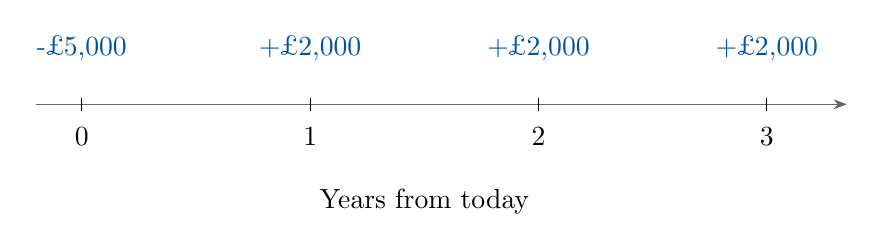
\begin{tikzpicture}[x=2.9cm,y=1cm,>=Stealth]
\draw[->,black!60] (-.2,0)--(3.35,0);
\foreach \t/\cash in {0/{-£5,000},1/{+£2,000},2/{+£2,000},3/{+£2,000}}{
\draw (\t,.08)--(\t,-.08);
\node[below=5pt] at (\t,0) {\t};
\node[above=12pt,text=StAndrewsBlue] at (\t,0) {\cash};}
\node[below=27pt] at (1.5,0) {Years from today};
\end{tikzpicture}
\end{center}
Date 0 is today. A minus sign is a payment; a plus sign is a receipt.
\end{frame}

\begin{frame}{Elements of a Timeline}
\begin{wideitemize}
\item Date (Time) 0 represents the present
\item Date 1 is one period from now and represents the end of Period 1 (year, quarter, month. . . )
\item Date 2 is two periods from now and represents the end of Period 2. . .
\item The space between Date 0 and Date 1 represents the time period between these two dates
\item Date 1 signifies \alert{both} the end of Period 1 and the beginning of Period 2
\end{wideitemize}
\end{frame}

\subsection{Rules of Time Travel}

\begin{frame}{Rules of Time Travel}
\begin{wideitemize}
\item Values can only be compared and combined if cash flows occur at the same point in time in the same unit
\begin{itemize}
\item £100 + \$100 = ?
\item €1 today + €1 tomorrow = ?
\end{itemize}
\item Moving cash flows forward = compounding (Eq.1)
\item Moving cash flows back in time = discounting (Eq.2)
\end{wideitemize}
\end{frame}

\begin{frame}{Discount each cash flow to the same date}
For equally spaced dates and a constant per-period discount rate:
\[
PV_0=\sum_{t=0}^{T}\frac{CF_t}{(1+r)^t}.
\]
\begin{itemize}
\item Include $CF_0$ without discounting; use signed net cash flows.
\item Match the rate to the timing, currency and risk of the cash flows.
\item For certain cash flows, the PV is the cost of a matching investment at the assumed rate. Risky expected cash flows require a risk-appropriate valuation.
\end{itemize}
\end{frame}

\begin{frame}{Example 1}
You have just graduated and need money to buy a new car. Your rich Uncle Richard will lend you the money so long as you agree to pay him back within five years, and you offer to pay him a rate of interest that he would otherwise get by putting his money in a savings account.

Based on your expected earnings and living expenses, you think you will be able to pay him £3,200 in one year; £3,500 in two years; £4,100 in three years; £5,500 in four years and £7,000 in five years.

If your uncle would otherwise earn 3\% per year on his savings, how much can you borrow from him today? Verify your answer by calculating the future value of this stream of cash flows.
\end{frame}

\begin{frame}{Discount the five promised repayments}
Assume year-end payments and a 3\% annual rate appropriate to this loan.
\[
PV_0=\frac{3200}{1.03}+\frac{3500}{1.03^2}+\frac{4100}{1.03^3}
       +\frac{5500}{1.03^4}+\frac{7000}{1.03^5}
\]
\[
\boxed{PV_0=\text{£}\UnclePV}
\]
This is less than the £23,300 sum of promised payments.

\smallskip
In practice, a risky family loan need not have the same required return as a bank deposit.
\end{frame}

\begin{frame}{Both routes give the same value in year 5}
\begin{block}{Invest the present value today}
\[FV_5=PV_0(1.03)^5=\text{£}\UncleFV\]
\end{block}
\begin{block}{Reinvest each repayment until year 5}
\[FV_5=3200(1.03)^4+3500(1.03)^3+4100(1.03)^2+5500(1.03)+7000\]
\[=\text{£}\UncleFV\]
\end{block}
Keep full precision in the calculation; round the displayed answer only.
\end{frame}

\subsection{Quoted and Effective Rates}

\begin{frame}{Distinguish a nominal quote from UK APR and AER}
\begin{wideitemize}
\item A \textbf{nominal annual rate} $j$, compounded $m$ times a year, gives a periodic rate of $j/m$. This is the convention used in our compounding formula.
\item UK consumer \textbf{APR (annual percentage rate)} is an annual measure of borrowing cost, including relevant compulsory charges. It is not simply $j$.
\item \textbf{AER (annual equivalent rate)} expresses savings interest on an annual basis, allowing for compounding.
\item Discount using an effective rate for the cash-flow period. Do not divide a UK consumer APR by $m$ as if it were a nominal quote.
\end{wideitemize}
\source{UK terminology: \href{https://www.moneyhelper.org.uk/en/savings/types-of-savings/how-to-choose-between-saving-and-borrowing}{MoneyHelper, choosing between saving and borrowing}.}
\end{frame}

\begin{frame}{Convert a nominal quote into an effective annual rate}
Let $j$ be the nominal annual rate, $m$ the number of compounding periods per year, and $n$ the number of years.
\[
FV_n=PV_0\left(1+\frac{j}{m}\right)^{mn}
      =PV_0(1+r_{\mathrm{annual}})^n
\]
\[
\boxed{r_{\mathrm{annual}}=\left(1+\frac{j}{m}\right)^m-1}
\]
For monthly cash flows, use $j/12$; for annual cash flows, use $r_{\mathrm{annual}}$.

With a fixed savings rate and this compounding convention, the annual result is the AER.
\end{frame}

\begin{frame}{More frequent compounding raises the annual return}
Fixed \textbf{nominal annual rate $j=10\%$}; no fees or withdrawals.
\begin{center}\begin{tabular}{lr}\toprule
Compounding & Effective annual rate\\\midrule
Annual & 10.000\%\\
Semi-annual & 10.250\%\\
Quarterly & 10.381\%\\
Monthly & 10.471\%\\
Weekly & 10.506\%\\
Daily & 10.516\%\\
Continuous & 10.517\%\\
\bottomrule\end{tabular}
\end{center}
The continuous-compounding limit is $e^{0.10}-1=10.517\%$.
\end{frame}

\subsection{Inflation and the Time Value of Money}

\begin{frame}{Match nominal cash flows with nominal discount rates}
\begin{columns}[T,onlytextwidth]
\column{0.46\textwidth}
\begin{block}{Nominal valuation}
Cash flows in the money of their payment date.\\
Discount at a nominal rate.
\end{block}
\column{0.46\textwidth}
\begin{block}{Real valuation}
Cash flows in constant purchasing-power units.\\
Discount at a real rate.
\end{block}
\end{columns}
\[
1+r_{\mathrm{real}}=\frac{1+r_{\mathrm{nominal}}}{1+\pi}
\]
The two valuations agree when cash flows and rates use the same inflation assumption. Here $\pi$ is a constant, known inflation rate; uncertain inflation requires additional care.
\end{frame}

\begin{frame}{Nominal and real calculations give the same present value}
Nominal interest rate = 3\%; inflation = 2\%. The payment is \$100 in one year, measured in that year's money.
\[
PV_0=\frac{100}{1.03}=\$97.09
\]
In today's purchasing-power units:
\[
CF_{1,\mathrm{real}}=\frac{100}{1.02}=\$98.0392,\qquad
r_{\mathrm{real}}=\frac{1.03}{1.02}-1=0.9804\%.
\]
\[
PV_0=\frac{100/1.02}{1.03/1.02}=\$97.09.
\]
\end{frame}

\subsection{Perpetuities and Annuities}

\begin{frame}{A level perpetuity begins one period after its valuation date}
\begin{wideitemize}
\item An equal payment $C$ arrives at each period-end forever.
\item With a constant per-period discount rate $r>0$:
\[PV_0=\frac{C}{r}.\]
\item The first payment is at date 1. If it starts later, discount this value back from one period before the first payment.
\item British consols are a historical example of undated government debt; the remaining UK undated gilts were redeemed in 2015.
\end{wideitemize}
\source{Historical context: \href{https://www.gov.uk/government/news/repayment-of-26-billion-historical-debt-to-be-completed-by-government}{HM Treasury, 27 March 2015}.}
\end{frame}

\begin{frame}{Constant growth requires a discount rate above growth}
Payments begin at date 1 and grow at the constant per-period rate $g$:
\[
C_t=C_1(1+g)^{t-1},\qquad PV_0=\frac{C_1}{r-g}.
\]
\begin{itemize}
\item $C_1$ is the \textbf{next} payment, not a payment today.
\item For positive payments and $r,g>-1$, convergence requires $r>g$.
\item At $g\geq r$, the positive-payment infinite sum does not converge to a finite PV. Do not use the formula to report a negative value.
\item Constant growth, constant risk and an infinite horizon are modelling assumptions, not forecasts to take literally.
\end{itemize}
\end{frame}

\begin{frame}{An ordinary annuity pays at the end of each period}
$N$ equal payments $C$ occur at dates $1,\ldots,N$; $r$ is the matching per-period rate.
\[
PV_0=\frac{C}{r}\left[1-(1+r)^{-N}\right],\qquad
FV_N=\frac{C}{r}\left[(1+r)^N-1\right].
\]
\begin{itemize}
\item The future value is measured immediately after the final payment.
\item For an annuity due (payments at $0,\ldots,N-1$), multiply the ordinary-annuity PV by $(1+r)$.
\item At $r=0$, both values are simply $NC$.
\end{itemize}
\end{frame}

\subsection{Common Mistakes}

\begin{frame}{Value the stream one period before its first payment}
\begin{center}\begin{tikzpicture}[x=2.6cm,y=1cm,>=Stealth]
\draw[->,black!60] (-.2,0)--(4.35,0);
\draw[line width=3pt,white] (.44,0)--(.56,0);
\draw[black!60] (.44,-.07)--(.48,.07) (.52,-.07)--(.56,.07);
\foreach \x/\t in {0/0,1/{k-1},2/k,3/{k+1},4/{k+2}}{
\draw (\x,.07)--(\x,-.07);\node[below=5pt] at (\x,0) {$\t$};}
\foreach \x in {2,3,4}{\node[above=12pt,text=StAndrewsBlue] at (\x,0) {$C$};}
\node[above=12pt,text=StAndrewsBurgundy] at (1,0) {$PV_{k-1}$};
\draw[->,StAndrewsBurgundy] (1,-.95)--(0,-.95) node[midway,below=5pt] {Discount back};
\end{tikzpicture}
\end{center}
For a stream beginning at date $k$, the standard formula gives $PV_{k-1}$.
\[
PV_0=\frac{PV_{k-1}}{(1+r)^{k-1}}.
\]
The date of the first payment determines how far to discount back.
\end{frame}

\begin{frame}{A first payment in year 2 gives a value in year 1}
An alumnus funds a £5,000 annual Business School graduation party forever. Assume a constant 12\% annual investment return; the first party is in two years.
\begin{center}\begin{tikzpicture}[x=2.6cm,y=1cm,>=Stealth]
\draw[->,black!60] (-.2,0)--(4.35,0);
\foreach \x/\t in {0/0,1/1,2/2,3/3,4/{\cdots}}{
\draw (\x,.07)--(\x,-.07);\node[below=5pt] at (\x,0) {$\t$};}
\foreach \x in {2,3}{\node[above=12pt,text=StAndrewsBlue] at (\x,0) {£5,000};}
\node[above=12pt,text=StAndrewsBurgundy] at (1,0) {$PV_1=C/r$};
\draw[->,StAndrewsBurgundy] (1,-.85)--(0,-.85) node[midway,below=5pt] {$\div\,1.12$};
\end{tikzpicture}
\end{center}
\[
PV_1=\frac{5000}{0.12}=\text{£}41,666.67,\qquad
PV_0=\frac{5000/0.12}{1.12}=\boxed{\text{£}37,202.38}.
\]
The 12\% return is an exercise assumption, not a guaranteed endowment yield.
\end{frame}

\begin{frame}{Five payments from year 7 are first valued in year 6}
Roberta Balotelli receives €1,000 each year at dates 7--11. The annual discount rate is 3\%.
\begin{center}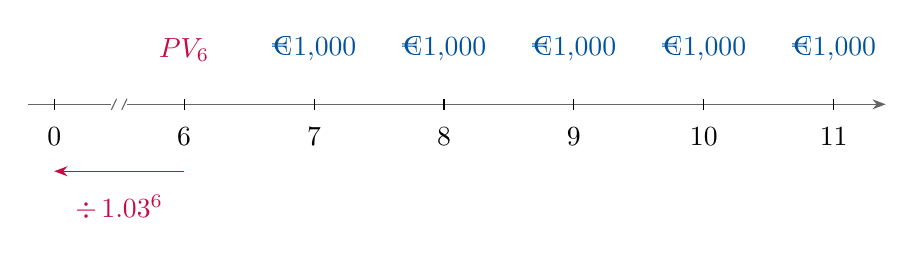
\begin{tikzpicture}[x=1.65cm,y=1cm,>=Stealth]
\draw[->,black!60] (-.2,0)--(6.4,0);
\draw[line width=3pt,white] (.44,0)--(.56,0);
\draw[black!60] (.44,-.07)--(.48,.07) (.52,-.07)--(.56,.07);
\foreach \x/\t in {0/0,1/6,2/7,3/8,4/9,5/10,6/11}{
\draw (\x,.07)--(\x,-.07);\node[below=5pt] at (\x,0) {$\t$};}
\foreach \x in {2,3,4,5,6}{\node[above=12pt,text=StAndrewsBlue] at (\x,0) {€1,000};}
\node[above=12pt,text=StAndrewsBurgundy] at (1,0) {$PV_6$};
\draw[->,StAndrewsBurgundy] (1,-.85)--(0,-.85) node[midway,below=5pt] {$\div\,1.03^6$};
\end{tikzpicture}
\end{center}
\[
PV_6=\frac{1000}{0.03}\left[1-1.03^{-5}\right]=\text{€}4,579.71
\]
\[
PV_0=\frac{PV_6}{1.03^6}=\boxed{\text{€}3,835.43}.
\]
\end{frame}

\section[Part 2: Investment Appraisal]{\textbf{Part 2: Investment Appraisal}}

\subsection{Reading}

\begin{frame}{Required and further reading}
\textbf{Required}
\begin{itemize}
\item Hillier, Ross, Westerfield, Jaffe \& Jordan (2020), \textit{Corporate Finance}, 4th ed., Chapter 6: Net Present Value and Other Investment Rules.
\item Brealey, Myers, Allen \& Edmans (2023), \textit{Principles of Corporate Finance}, 14th ed., Chapters 5--6.
\item Graham \& Harvey (2001), \href{https://doi.org/10.1016/S0304-405X(01)00044-7}{The Theory and Practice of Corporate Finance: Evidence from the Field}. \textit{Journal of Financial Economics} 60, 187--243.
\end{itemize}
\textbf{Further reading}
\begin{itemize}
\item Graham (2022), \href{https://doi.org/10.1111/jofi.13161}{Presidential Address: Corporate Finance and Reality}. \textit{Journal of Finance} 77, 1975--2049.
\item Andor, Mohanty \& Toth (2015), \href{https://doi.org/10.1016/j.ememar.2015.04.002}{Capital Budgeting Practices: A Survey of Central and Eastern European Firms}. \textit{Emerging Markets Review} 23, 148--172.
\end{itemize}
\end{frame}

\subsection{Net Present Value}

\begin{frame}{NPV measures value created at the valuation date}
Net present value is the sum of all signed, incremental project cash flows discounted to date 0:
\[
NPV=CF_0+\sum_{t=1}^{T}\frac{\mathbb{E}[CF_t]}{(1+r)^t}.
\]
\begin{wideitemize}
\item Accept an independent project if $NPV>0$, subject to relevant constraints.
\item Among feasible, mutually exclusive alternatives, choose the highest NPV (including doing nothing).
\item Include taxes, working capital, opportunity costs and terminal obligations where relevant. The exercises simplify these inputs.
\end{wideitemize}
\end{frame}

\begin{frame}{The NPV Rule - Example 1}
In a hypothetical teaching case, Barrick Gold considers investing in a new gold mine in South Africa. Gold in South Africa is buried very deep, so the mine will require an initial investment of \$150 million. If this money is spent immediately, the mine is expected to produce revenues of \$30 million per year for 20 years, with the first cash flow coming one year from today. It will cost \$10 million per year to operate the mine, with the first cash outflow also occurring in one year's time. After 20 years, the gold will be depleted. The mine must then be stabilized on an ongoing basis, which will cost \$5 million per year forever \alert{with the first closure payment at date 21}.

Assuming that the cost of capital for Barrick Gold is 15\%, calculate the NPV of this project.
\end{frame}

\begin{frame}{Operating gains do not cover construction and closure}
All values are in \$ million. Operations pay $30-10=20$ at dates 1--20; closure costs begin at date 21.
\begin{block}{1. Discount the operating annuity}
\[PV_{\mathrm{operations}}=\frac{20}{0.15}(1-1.15^{-20})=\MineIn\]
\end{block}
\begin{block}{2. Include initial investment and the delayed perpetuity}
\[PV_{\mathrm{costs}}=150+\frac{5/0.15}{1.15^{20}}=\MineOut\]
\end{block}
\[NPV=\MineIn-\MineOut=-\$\MineNPV\text{ million: reject.}\]
\end{frame}

\begin{frame}{Match the discount rate to the cash flow being valued}
\textbf{Next lecture develops the cost of capital.}
\begin{wideitemize}
\item Match currency, inflation treatment, timing and risk. A government bond yield is a starting point for the risk-free component, not the project's whole required return.
\item CAPM estimates a cost of equity from a risk-free rate, beta and an equity risk premium. Firm cash flows generally require a financing-consistent cost of capital such as WACC.
\item A single rate is a useful simplification. With a term structure, discount each dated cash flow using its maturity-specific discount factor.
\item Spot rates and forward rates are related, but neither makes future reinvestment returns certain.
\end{wideitemize}
\end{frame}

\begin{frame}{Economic Rents and NPV}
\begin{wideitemize}
\item Profits that more than cover the opportunity cost of capital are known as economic rents
\item Think about competitive advantage
\end{wideitemize}
\end{frame}

\subsection{The IRR Rule}

\begin{frame}{The IRR rule works for conventional independent investments}
The internal rate of return solves
\[0=\sum_{t=0}^{T}\frac{CF_t}{(1+IRR)^t}.\]
\begin{wideitemize}
\item For one initial outflow followed by non-negative inflows (at least one positive), the NPV profile decreases with the rate and has a unique IRR for $r>-1$.
\item With a constant appropriate required return, accept an independent conventional investment when $IRR>r$.
\item For mutually exclusive projects, reversed signs, multiple sign changes or differing discount rates, return to NPV.
\end{wideitemize}
\end{frame}

\begin{frame}{The IRR Rule - Example 2}
Suppose that you are in the real estate business. You are considering the construction of an office block to let. You have been approached by a potential tenant who is prepared to rent your office block for 5 years at a fixed annual rent of £35,000. The construction would cost you £750,000 and the office block would be ready to let one year from now if work starts immediately. You predict that 6 years from now you will be able to sell the office block for £1,125,500. Assume the rent is paid annually at the beginning of each year and your opportunity cost of capital is 9\%. Is the construction a worthwhile investment?
\end{frame}

\begin{frame}{Rent begins at date 1; the sale occurs at date 6}
Construction is paid now. Five rents are paid in advance at dates 1--5 for occupancy during years 2--6; there is no additional rent at date 6.
\begin{center}
\begin{tabular}{lrrrrrrr}\toprule
Date & 0 & 1 & 2 & 3 & 4 & 5 & 6\\\midrule
Cash flow (£000) & -750 & 35 & 35 & 35 & 35 & 35 & 1,125.5\\
\bottomrule\end{tabular}

\end{center}
\[0=-750000+35000\sum_{t=1}^{5}(1+IRR)^{-t}+1125500(1+IRR)^{-6}.\]
Solve numerically; then check the root by substituting it into the NPV equation.
\end{frame}

\begin{frame}{1. Find two rates with NPVs on opposite sides of zero}
We want the discount rate that makes the office development's \textbf{NPV equal to zero}.
\medskip
\begin{columns}[T,onlytextwidth]
\column{0.46\textwidth}
\begin{block}{Try a discount rate of 10\%}
{\large\color{StAndrewsBlue}NPV = +£\InterpPositive}

Still positive: the rate needs to \textbf{rise}.
\end{block}
\column{0.46\textwidth}
\begin{block}{Try a discount rate of 10.5\%}
{\large\color{StAndrewsBurgundy}NPV = −£\InterpNegative}

Now negative: we have \textbf{gone too far}.
\end{block}
\end{columns}
\medskip
The IRR lies between 10\% and 10.5\%. \textbf{Interpolation estimates how far across this interval we need to move.}

We approximate the NPV curve by a straight line between these two nearby trial results.
\end{frame}

\begin{frame}{2. First, see the idea with easy numbers}
\textbf{A separate illustration:} suppose NPV falls from +£300 to −£100 as the rate rises from 10\% to 10.5\%. Assume a straight line between the results.
\begin{center}% A linear illustration, not a new set of office-project cash flows.
\begin{tikzpicture}[x=1cm,y=1cm]
\foreach \y in {0,1.45}{
  \draw[black!40,line width=1pt] (0,\y)--(10,\y);
  \draw[StAndrewsBlue,line width=2pt] (0,\y)--(\InterpToyPosition,\y);
  \foreach \x in {0,\InterpToyPosition,10}{\draw[black!65] (\x,\y-.07)--(\x,\y+.07);}
}
\node[anchor=east] at (-.4,1.45) {NPV};
\node[anchor=east] at (-.4,0) {Rate};
\node[below=6pt,anchor=north west] at (0,1.45) {+£300};
\node[below=6pt,anchor=north east] at (10,1.45) {−£100};
\node[above=7pt,text=StAndrewsBlue] at (\InterpToyPosition,1.45) {£0};
\node[below=6pt,anchor=north west] at (0,0) {10\%};
\node[below=6pt,anchor=north east] at (10,0) {10.5\%};
\node[above=7pt,text=StAndrewsBlue] at (\InterpToyPosition,0) {10.375\%};
\node[above=7pt,text=StAndrewsBlue] at (3,1.45) {Three-quarters of the fall};
\node[above=7pt,text=StAndrewsBlue] at (3,0) {Three-quarters of the rate gap};
\end{tikzpicture}
\end{center}
The full NPV fall is £400. Reaching zero uses £300 of it: \textbf{three-quarters of the fall}.
\[
\text{Estimated rate}=10\%+\underbrace{\frac{300}{400}}_{\text{three-quarters}}\times
\underbrace{(10.5\%-10\%)}_{\text{full rate interval}}=10.375\%.
\]
\end{frame}

\begin{frame}{3. For the office project, zero uses 96.05 per cent of the fall}
Return to our actual trial NPVs: +£\InterpPositive\ and −£\InterpNegative.
\begin{block}{How far does NPV fall across the whole interval?}
\[
\InterpPositive-(-\InterpNegative)=\text{£}\InterpFall
\]
We pass zero and then fall another £\InterpNegative, so \textbf{add the two magnitudes}.
\end{block}
\begin{block}{How much of that fall takes us just to zero?}
\[
\text{Fraction needed}=\frac{\InterpPositive}{\InterpFall}=\InterpFractionDecimal\approx\InterpFractionPercent\%.
\]
\end{block}
We need almost the whole fall: the estimated IRR should be \textbf{close to 10.5\%}.
\end{frame}

\begin{frame}{4. Move the same fraction of the way from 10 to 10.5 per cent}
A straight line means equal rate increases produce equal NPV falls. So \textbf{96.05\% of the NPV fall corresponds to 96.05\% of the rate interval}.
\begin{center}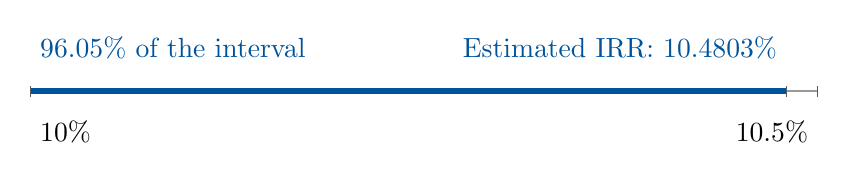
\begin{tikzpicture}[x=1cm,y=1cm]
\draw[black!40,line width=1pt] (0,0)--(10,0);
\draw[StAndrewsBlue,line width=2pt] (0,0)--(\InterpRatePosition,0);
\foreach \x in {0,\InterpRatePosition,10}{\draw[black!65] (\x,-.07)--(\x,.07);}
\node[below=7pt,anchor=north west] at (0,0) {10\%};
\node[below=7pt,anchor=north east] at (10,0) {10.5\%};
\node[above=8pt,anchor=south east,text=StAndrewsBlue] at (\InterpRatePosition,0) {Estimated IRR: \InterpRateFour\%};
\node[above=8pt,anchor=south west,text=StAndrewsBlue] at (0,0) {\InterpFractionPercent\% of the interval};
\end{tikzpicture}
\end{center}
\[
\begin{aligned}
\text{Full rate interval}&=10.5\%-10\%=0.5\text{ percentage points}\\
\text{Increase needed}&=\InterpFractionDecimal\times0.5\approx\InterpRateIncrease\text{ percentage points}\\
\text{Estimated IRR}&=10\%+\InterpRateIncrease\%=\boxed{\InterpRateFour\%}.
\end{aligned}
\]
Start at 10\%, then add \textbf{part of the 0.5-point gap}. Do not multiply 10\% by the fraction.
\end{frame}

\begin{frame}{5. The formula simply records those three steps}
\[
\boxed{\text{Estimated IRR}=\text{starting rate}+\text{fraction needed}\times\text{rate interval}}
\]
Let $r_L$ be the lower trial rate, with $NPV_L>0$, and $r_H$ the higher trial rate, with $NPV_H<0$.
\[
IRR\approx
\underbrace{r_L}_{\text{start}}+
\underbrace{\frac{NPV_L}{NPV_L-NPV_H}}_{\text{fraction of NPV fall}}\times
\underbrace{(r_H-r_L)}_{\text{rate interval}}.
\]
\begin{itemize}
\item The denominator is the \textbf{full fall in NPV}, not just the negative endpoint.
\item If you write the endpoints as $+A$ and $-B$, that fraction is $A/(A+B)$.
\item Check that the fraction lies between 0 and 1, and the answer between your two trial rates.
\end{itemize}
\end{frame}

\begin{frame}{6. Check the estimate: the NPV curve is not exactly straight}
\begin{center}\begin{tikzpicture}
\begin{axis}[lectureplot,width=10.4cm,height=3.6cm,xmin=10,xmax=10.5,ymin=-3,ymax=20,
xtick={10,10.25,10.5},ytick={0,10,20},xlabel={Discount rate (\%)},ylabel={NPV (£000)}]
\addplot[black!35,thin] coordinates {(10,0)(10.5,0)};
\addplot[StAndrewsBlue] table[x=rate,y=office]{generated/interpolation.dat};
\addplot[StAndrewsBurgundy,dashed] table[x=rate,y=npv]{generated/interp_segment.dat};
\node[font=\footnotesize,anchor=south west,text=StAndrewsBurgundy] at (axis cs:10.17,14) {Straight-line approximation};
\node[font=\footnotesize,anchor=south west,text=StAndrewsBlue] at (axis cs:10.03,3.5) {NPV curve};
\end{axis}\end{tikzpicture}
\end{center}
Interpolation gives \textbf{\InterpRateFive\%}; a numerical solver gives \textbf{\InterpRootFive\%}. Both round to \textbf{10.48\%}.

Substituting the unrounded interpolation estimate gives NPV $\approx-\text{£}\InterpResidualWhole$, close to zero. The straight line gives a small approximation error.

Use nearby trial rates for interpolation; use a spreadsheet IRR function or a numerical solver when you need greater precision.
\end{frame}

\begin{frame}{The office development creates value at 9 per cent}
\begin{center}\begin{tikzpicture}
\begin{axis}[lectureplot,xmin=0,xmax=25,ymin=-400,ymax=600,
xtick={0,5,10,15,20,25},ytick={-400,-200,0,200,400,600},xlabel={Discount rate (\%)},ylabel={NPV (£000)}]
\addplot[black!35,thin] coordinates {(0,0)(25,0)};
\addplot[StAndrewsBlue] table[x=rate,y=office]{generated/office.dat};
\addplot[only marks,mark=*,mark size=2pt,StAndrewsBurgundy] table[x=rate,y=npv]{generated/office_point.dat};
\node[font=\small,anchor=south west,text=StAndrewsBlue] at (axis cs:12,200) {Office development};
\node[font=\footnotesize,anchor=south west] at (axis cs:9.8,65) {9\% required return};
\end{axis}\end{tikzpicture}
\end{center}
At 9\%, $NPV=\text{£}\OfficeNPV$; the zero crossing is $IRR=\OfficeIRR\%$.
\end{frame}

\subsection{IRR Rule Limitations}

\begin{frame}{The IRR Rule Limitations}
\begin{wideitemize}
\item Mutually exclusive projects (MEPs) are alternatives: choosing one rules out the others.
\item Choose the feasible alternative with the highest NPV, including doing nothing. What would the IRR rule suggest?
\item Would it make sense to choose the project with the highest IRR?
\end{wideitemize}
\end{frame}

\begin{frame}{Example 3: the higher IRR need not give the higher NPV}
An alternative is to sell the office block immediately on completion at date 1 for £862,500. Construction still costs £750,000 today.
\begin{center}\begin{tabular}{lrr}\toprule
Project & IRR & NPV at 9\%\\\midrule
1: let, then sell & 10.48\% & £57,236.67\\
2: sell on completion & 15.00\% & £41,284.40\\
\bottomrule\end{tabular}
\end{center}
At 9\%, choose Project 1 if these are mutually exclusive alternatives with the same relevant risk and no other constraints.
\end{frame}

\begin{frame}{The preferred project changes at the crossover rate}
\begin{center}\begin{tikzpicture}
\begin{axis}[lectureplot,xmin=0,xmax=20,ymin=-300,ymax=600,
xtick={0,5,10,15,20},ytick={-200,0,200,400,600},xlabel={Discount rate (\%)},ylabel={NPV (£000)}]
\addplot[black!35,thin] coordinates {(0,0)(20,0)};
\addplot[StAndrewsBlue] table[x=rate,y=office]{generated/ranking.dat};
\addplot[StAndrewsBurgundy,dashed] table[x=rate,y=sell]{generated/ranking.dat};
\addplot[only marks,mark=*,mark size=2pt,black] table[x=rate,y=npv]{generated/ranking_cross.dat};
\node[font=\small,anchor=south west,text=StAndrewsBlue] at (axis cs:2,470) {1: let, then sell};
\node[font=\small,anchor=south west,text=StAndrewsBurgundy] at (axis cs:12,110) {2: sell at date 1};
\end{axis}\end{tikzpicture}
\end{center}
The NPV profiles cross at \CrossRate\%. At 9\%, letting then selling creates more value.
\end{frame}

\begin{frame}{NPV scales with investment; IRR does not}
\begin{wideitemize}
\item IRR is a percentage rate; NPV measures value created in currency units.
\item If every office-development cash flow doubles, NPV doubles to £\DoubleNPV\ at 9\%.
\item The IRR remains \OfficeIRR\% because multiplying the NPV equation by two leaves its zero unchanged.
\item This assumes an exact, feasible replication with the same risk and unit economics. Higher percentage returns alone cannot rank projects of different sizes.
\end{wideitemize}
\end{frame}

\begin{frame}{The Timing Problem (1.3) - MEPs}
\begin{wideitemize}
\item IRR can be altered by changing the timing of the cash flows, even when that change in timing does not affect the NPV
\item Therefore, it is possible to alter the ranking of projects' IRR without changing their ranking in terms of NPV
\end{wideitemize}
\end{frame}

\begin{frame}{NPV is Unchanged - Example 4}
Michael wants to start a laundry service for which he would need to invest £20,000 to buy the washers and dryers. He is comparing two stylised perpetual net cash-flow streams; ignore taxes, replacement costs and resale value.

\textbf{Option 1:} With self-maintenance, the net cash flow is £8,000 at date 1, then declines by 20\% each year forever.

\textbf{Option 2:} Alternatively, a maintenance contract sustains £8,000 before maintenance each year, and costs £5,000 at each year-end forever: net cash flow is £3,000.

Michael has an opportunity cost of capital of 12\% and the first cash inflow occurs one year from now if Michael starts his business immediately.

Compare the NPV and IRR of the two options.
\end{frame}

\begin{frame}{Equal NPVs at 12 per cent coexist with different IRRs}
\begin{columns}[T,onlytextwidth]
\column{0.47\textwidth}
\begin{block}{1. Self-maintenance: $g=-20\%$}
\[NPV_1=\frac{8000}{0.12+0.20}-20000\]
\[=\text{£}5,000,\qquad IRR_1=20\%.\]
\end{block}
\column{0.47\textwidth}
\begin{block}{2. Maintenance contract: $g=0$}
\[NPV_2=\frac{3000}{0.12}-20000\]
\[=\text{£}5,000,\qquad IRR_2=15\%.\]
\end{block}
\end{columns}
Michael is indifferent on NPV at 12\%, given the stated assumptions.
\end{frame}

\begin{frame}{The maintenance alternatives cross at 12 per cent}
\begin{center}\begin{tikzpicture}
\begin{axis}[lectureplot,xmin=5,xmax=30,ymin=-12,ymax=42,
xtick={5,10,15,20,25,30},ytick={-10,0,10,20,30,40},xlabel={Discount rate (\%)},ylabel={NPV (£000)}]
\addplot[black!35,thin] coordinates {(5,0)(30,0)};
\addplot[StAndrewsBlue] table[x=rate,y=self]{generated/maintenance.dat};
\addplot[StAndrewsBurgundy,dashed] table[x=rate,y=contract]{generated/maintenance.dat};
\addplot[only marks,mark=*,mark size=2pt,black] coordinates {(12,5)};
\node[font=\small,anchor=south west,text=StAndrewsBlue] at (axis cs:18,8) {Self-maintenance};
\node[font=\small,anchor=south west,text=StAndrewsBurgundy] at (axis cs:9,28) {Maintenance contract};
\end{axis}\end{tikzpicture}
\end{center}
Below 12\%, prefer the contract; above 12\%, self-maintenance has the higher NPV. Accept an investment only if its NPV is also positive.
\end{frame}

\begin{frame}{A crossover is the IRR of the difference in cash flows}
\begin{wideitemize}
\item Subtract one alternative's dated cash flows from the other's, then solve $NPV_{\mathrm{difference}}=0$.
\item The office alternatives cross at \CrossRate\%; the maintenance alternatives cross at 12\%.
\item A crossover helps locate where rankings change. Inspect which side has the higher NPV; the usual accept-if-higher IRR rule need not apply to the difference.
\item Use a common discount rate only if appropriate to the risks of both alternatives. Incremental cash flows may themselves have multiple or no IRRs.
\end{wideitemize}
\end{frame}

\begin{frame}{Multiple IRRs (2) - Example 5}
In a hypothetical case, King Coal Corporation is considering a project to strip-mine coal. The project requires an investment of \$210 million and is expected to produce a cash inflow (at the end of each year) of \$125 million in the first two years, building up to \$175 million each year in years 3 and 4. However, the company is obliged in year 5 to reclaim the land at a cost of \$400 million. The opportunity cost of capital of King Coal is 20\%.

Find the IRR of this project.

At 20\%: NPV = \$\CoalNPV\ million
\end{frame}

\begin{frame}{Two zero crossings make a single IRR misleading}
\begin{center}\begin{tikzpicture}
\begin{axis}[lectureplot,xmin=0,xmax=50,ymin=-45,ymax=15,
xtick={0,10,20,30,40,50},ytick={-40,-20,0,10},xlabel={Discount rate (\%)},ylabel={NPV (\$ million)}]
\addplot[black!35,thin] coordinates {(0,0)(50,0)};
\addplot[StAndrewsBlue] table[x=rate,y=coal]{generated/coal.dat};
\addplot[only marks,mark=*,mark size=2pt,StAndrewsBurgundy] table[x=rate,y=npv]{generated/coal_point.dat};
\addplot[only marks,mark=*,mark size=2pt,black] table[x=rate,y=npv]{generated/coal_roots.dat};
\node[font=\small,anchor=south west,text=StAndrewsBlue] at (axis cs:29,6) {King Coal};
\end{axis}\end{tikzpicture}
\end{center}
IRRs: \CoalLowIRR\% and \CoalHighIRR\%. At 20\%, $NPV=\$\CoalNPV$ million: accept on NPV.
\end{frame}

\begin{frame}{Modified returns require an explicit convention}
\begin{wideitemize}
\item King Coal's signs are $-\,,+\,,+\,,+\,,+\,,-$: two sign changes. The number of admissible IRRs cannot exceed the sign changes; it can be smaller.
\item One approach discounts later negative cash flows back until the adjusted stream has just one sign change.
\item Conventional terminal-value MIRR instead discounts outflows to date 0 and compounds inflows to the final date, using specified finance and reinvestment rates.
\item These are different constructions and need not give the same percentage. NPV remains the valuation criterion.
\end{wideitemize}
\end{frame}

\begin{frame}{King Coal: discount later outflows back at 20 per cent}
All cash flows are in \$ million. Preserve their value at the 20\% required return.
\[
CF'_4=175-\frac{400}{1.20}=-158.33
\]
Still negative: combine dates 3--5 at date 3 instead.
\[
CF'_3=175+\frac{175}{1.20}-\frac{400}{1.20^2}=43.0556
\]
\[
0=-210+\frac{125}{1+r^*}+\frac{125}{(1+r^*)^2}+\frac{43.0556}{(1+r^*)^3}
\]
\textbf{Adjusted-cash-flow IRR = \CoalAdjustedIRR\%}. This exceeds 20\%, consistent with the original positive NPV; it is not the terminal-value MIRR.
\end{frame}


\begin{frame}{King Coal: conventional terminal-value MIRR is different}
Use a 20\% finance rate and 20\% reinvestment rate over the original five-year horizon (\$ million).
\[
PV_- =210+\frac{400}{1.20^5}=\CoalPVminus
\]
\[
FV_+ =125(1.20)^4+125(1.20)^3+175(1.20)^2+175(1.20)=\CoalFVplus
\]
\[
MIRR=\left(\frac{FV_+}{PV_-}\right)^{1/5}-1=\boxed{\CoalMIRR\%}.
\]
This also exceeds 20\%. Always state the rates, horizon and modification convention.
\end{frame}

\begin{frame}{Delayed Investments (3) - Example 6}
In this fictional example, John Star, the founder of SuperTech, has just retired as CEO. A major publisher has offered him a €1 million ``how I did it'' book deal. That is, the publisher will pay him €1 million upfront if Star agrees to write a book about his experiences. He estimates that it will take him three years to write the book. The time that he spends writing will cause him to forgo alternative sources of income amounting to €500,000 per year. Considering the risk of his alternative income sources and available investment opportunities, Star estimates his opportunity cost of capital to be 10\%.

Calculate the IRR of this project.
\end{frame}

\begin{frame}{The IRR Rule versus the IRR}
\begin{wideitemize}
\item IRR = 23.38\% > 10\%
\item But NPV = - €243,426
\item It is as if Star was borrowing money
\item IRR should be lower than the opportunity cost of capital for this project to be accepted
\item The IRR rule fails but the IRR itself still provides useful information in conjunction with the NPV rule
\end{wideitemize}
\end{frame}

\begin{frame}{Non-existent IRR (4) - Example 7}
Luckily for John Star, he has other opportunities available to him. An agent has approached him and guaranteed €1 million in each of the next three years if he will agree to give four lectures per month over that period. Star estimates that preparing and delivering the lectures would take the same amount of time as writing the book – that is, the cost would be €500,000 per year. What is the IRR of this opportunity?

$$\frac{(1 - 0.5)}{(1 + IRR)} + \frac{(1 - 0.5)}{(1 + IRR)^2} + \frac{(1 - 0.5)}{(1 + IRR)^3} = 0$$

At 10\%, NPV = €1,243,426. All cash flows are positive, so there is no finite IRR for $r>-1$. A stream of only negative cash flows would likewise have no IRR.
\end{frame}

\subsection{The Payback Period Rule}

\begin{frame}{The Payback Period Rule}
\begin{wideitemize}
\item The payback period is the length of time required for an investment to generate cash flows sufficient to recover its initial cost
\item Simple payback versus discounted payback
\item Based on the payback rule, an investment is acceptable if its payback period is less than a pre-specified number of years
\end{wideitemize}
\end{frame}

\begin{frame}{Example 8: payback depends on the timing convention}
Initial investment: ¥300 million; annual discount rate: 5\%. Table units: ¥ million.
\begin{center}\begin{tabular}{lrrrr}\toprule
Year & Cash flow & Cumulative & Discounted & Cumulative PV\\\midrule
1 & 100 & 100 & 95.24 & 95.24\\
2 & 150 & 250 & 136.05 & 231.29\\
3 & 150 & 400 & 129.58 & 360.87\\
\bottomrule\end{tabular}
\end{center}
With the usual within-year linear interpolation:
\[
SPB=2+\frac{300-250}{150}=2.33,\qquad
DPB=2+\frac{300-(100/1.05+150/1.05^2)}{150/1.05^3}=\DiscountedPB.
\]
If all receipts occur strictly at year-end, both payback dates are year 3. Fractional paybacks are approximations. Neither rule values cash flows after the cutoff.
\end{frame}

\subsection{The Average Accounting Return}

\begin{frame}{AAR compares accounting profit with average book value}
Average accounting return (\textbf{AAR}), also called accounting rate of return (ARR), uses accounting profit after tax and depreciation:
\[
AAR=\frac{\text{Average annual net income}}{\text{Average book value of the investment}}.
\]
\begin{itemize}
\item We use \textbf{AAR} consistently in this lecture and specify this denominator.
\item Compare it with an accounting-return target, not automatically the cost of capital.
\item It ignores cash-flow timing and depends on accounting conventions; it does not measure value creation.
\end{itemize}
\end{frame}

\begin{frame}{The AAR: Example 9}
Suppose we are deciding whether or not to open a store in a new shopping mall. The required investment in improvements is £500,000. The store would have a five-year life because everything reverts to the mall owners after that time. The required investment would be 100-percent depreciated using straight line depreciation. The tax rate is 25\%. The target return on new investments is 15\%.

Should the project be accepted?
\end{frame}

\begin{frame}{Calculate tax and net income before rounding}
Straight-line depreciation: £500,000 / 5 = £100,000 per year. Tax rate: 25\%.
\begin{center}\begin{tabular}{lrrrrr}\toprule
£ thousand & Year 1 & Year 2 & Year 3 & Year 4 & Year 5\\\midrule
Sales & 350 & 360 & 355 & 320 & 310\\
Expenses & 200 & 170 & 150 & 150 & 150\\
Before depreciation & 150 & 190 & 205 & 170 & 160\\
Depreciation & 100 & 100 & 100 & 100 & 100\\
Before tax & 50 & 90 & 105 & 70 & 60\\
Tax (25\%) & 12.5 & 22.5 & 26.25 & 17.5 & 15\\
Net income & 37.5 & 67.5 & 78.75 & 52.5 & 45\\
\bottomrule\end{tabular}
\end{center}
All table values are in £ thousand; taxes and income retain their exact quarter-thousand values.
\end{frame}

\begin{frame}{The average accounting return is 22.5 per cent}
\[
\overline{NI}=\frac{37{,}500+67{,}500+78{,}750+52{,}500+45{,}000}{5}=\text{£}56{,}250
\]
With straight-line depreciation to zero and no additional investment:
\[
\overline{BV}=\frac{500{,}000+0}{2}=\text{£}250{,}000
\]
\[
AAR=\frac{56{,}250}{250{,}000}=\boxed{22.5\%>15\%}.
\]
The project passes the stated AAR target. That result alone does not establish a positive NPV.
\end{frame}

\subsection{The Profitability Index}

\begin{frame}{State which profitability-index convention you use}
For an initial cost $I_0$ followed by inflows:
\[
PI_{\mathrm{benefit/cost}}=\frac{PV(\text{future inflows})}{I_0}
=1+\frac{NPV}{I_0}.
\]
\begin{itemize}
\item The benefit-cost convention accepts $PI>1$. A net index $NPV/I_0$ instead accepts values above zero.
\item Cost = \$10m and NPV = \$1m give a benefit-cost PI of \textbf{1.10}, or a net index of \textbf{0.10 (10\%)}.
\item Ranking by PI can help with divisible, independent projects under a single initial capital constraint. Indivisibility or multiple constraints require choosing the feasible combination with the highest total NPV.
\item PI does not reliably rank mutually exclusive projects of different scale. Later outflows also require an explicit denominator convention.
\end{itemize}
\end{frame}

\subsection{Capital Budgeting in Practice}

\begin{frame}{Firms commonly use several appraisal methods}
Reported ``always or almost always'' use, \textbf{March 2020 survey}.
\begin{center}\begin{tikzpicture}
\begin{axis}[lectureplot,width=10.7cm,height=3.7cm,xmin=0,xmax=105,ymin=.6,ymax=4.55,
xtick={0,25,50,75,100},ytick={1,2,3,4},
yticklabels={Profitability index,Payback,IRR/hurdle rate,NPV},xlabel={Per cent of firms},
axis y line=left,y axis line style={draw=none},ytick style={draw=none}]
\addplot[only marks,mark=*,mark size=2.3pt,StAndrewsBlue] table[x=large,y=y]{generated/survey.dat};
\addplot[only marks,mark=square*,mark size=2.2pt,StAndrewsBurgundy] table[x=small,y=y]{generated/survey.dat};
\node[font=\footnotesize,text=StAndrewsBlue,anchor=south] at (axis cs:80,4.35) {Large firms};
\node[font=\footnotesize,text=StAndrewsBurgundy,anchor=south] at (axis cs:40,4.35) {Small firms};
\end{axis}\end{tikzpicture}
\end{center}
\source{\href{https://doi.org/10.1111/jofi.13161}{Graham (2022), Table I, Panel A}, selected techniques. Table sample: 85 large and 376 small firms; US\$1bn annual-revenue threshold. Multiple responses allowed; percentages need not sum to 100.}
\end{frame}

\begin{frame}{Good appraisal combines valuation, uncertainty and feasibility}
\begin{wideitemize}
\item \textbf{Value:} estimate incremental cash flows and use NPV at a defensible discount rate. Identify the advantage that supports a positive forecast.
\item \textbf{Uncertainty:} challenge demand, costs, timing and terminal assumptions; use scenarios and sensitivity analysis to expose what could reverse the decision.
\item \textbf{Implementation:} assess resources, capabilities, stakeholder commitments and constraints alongside the valuation.
\item Make the assumptions and tradeoffs explicit, then review realised outcomes. Enthusiasm and consensus cannot substitute for a credible value case.
\end{wideitemize}
\end{frame}


\begin{frame}{Compare cash flows at a common date; use NPV to assess value}
\begin{center}
{\large\color{StAndrewsBlue}Timing first. Valuation second. Decision with judgement.}

\bigskip
Bring questions about the examples or your working to my office hours.
\end{center}
\end{frame}


\end{document}
